% !tex encoding = utf-8 unicode
\documentclass{book}
\usepackage{graphicx}
\usepackage{hyperref}
\usepackage{pdfpages}
\hypersetup{colorlinks=true,linkcolor=cyan,urlcolor=cyan}
\usepackage[letterpaper, margin=1in]{geometry}
\graphicspath{ {../img/} }
\setcounter{secnumdepth}{-1}

\title{curriculum vitae}
\author{fede camara halac}
\date{march 2017}

\begin{document}

\maketitle
\section {personal}
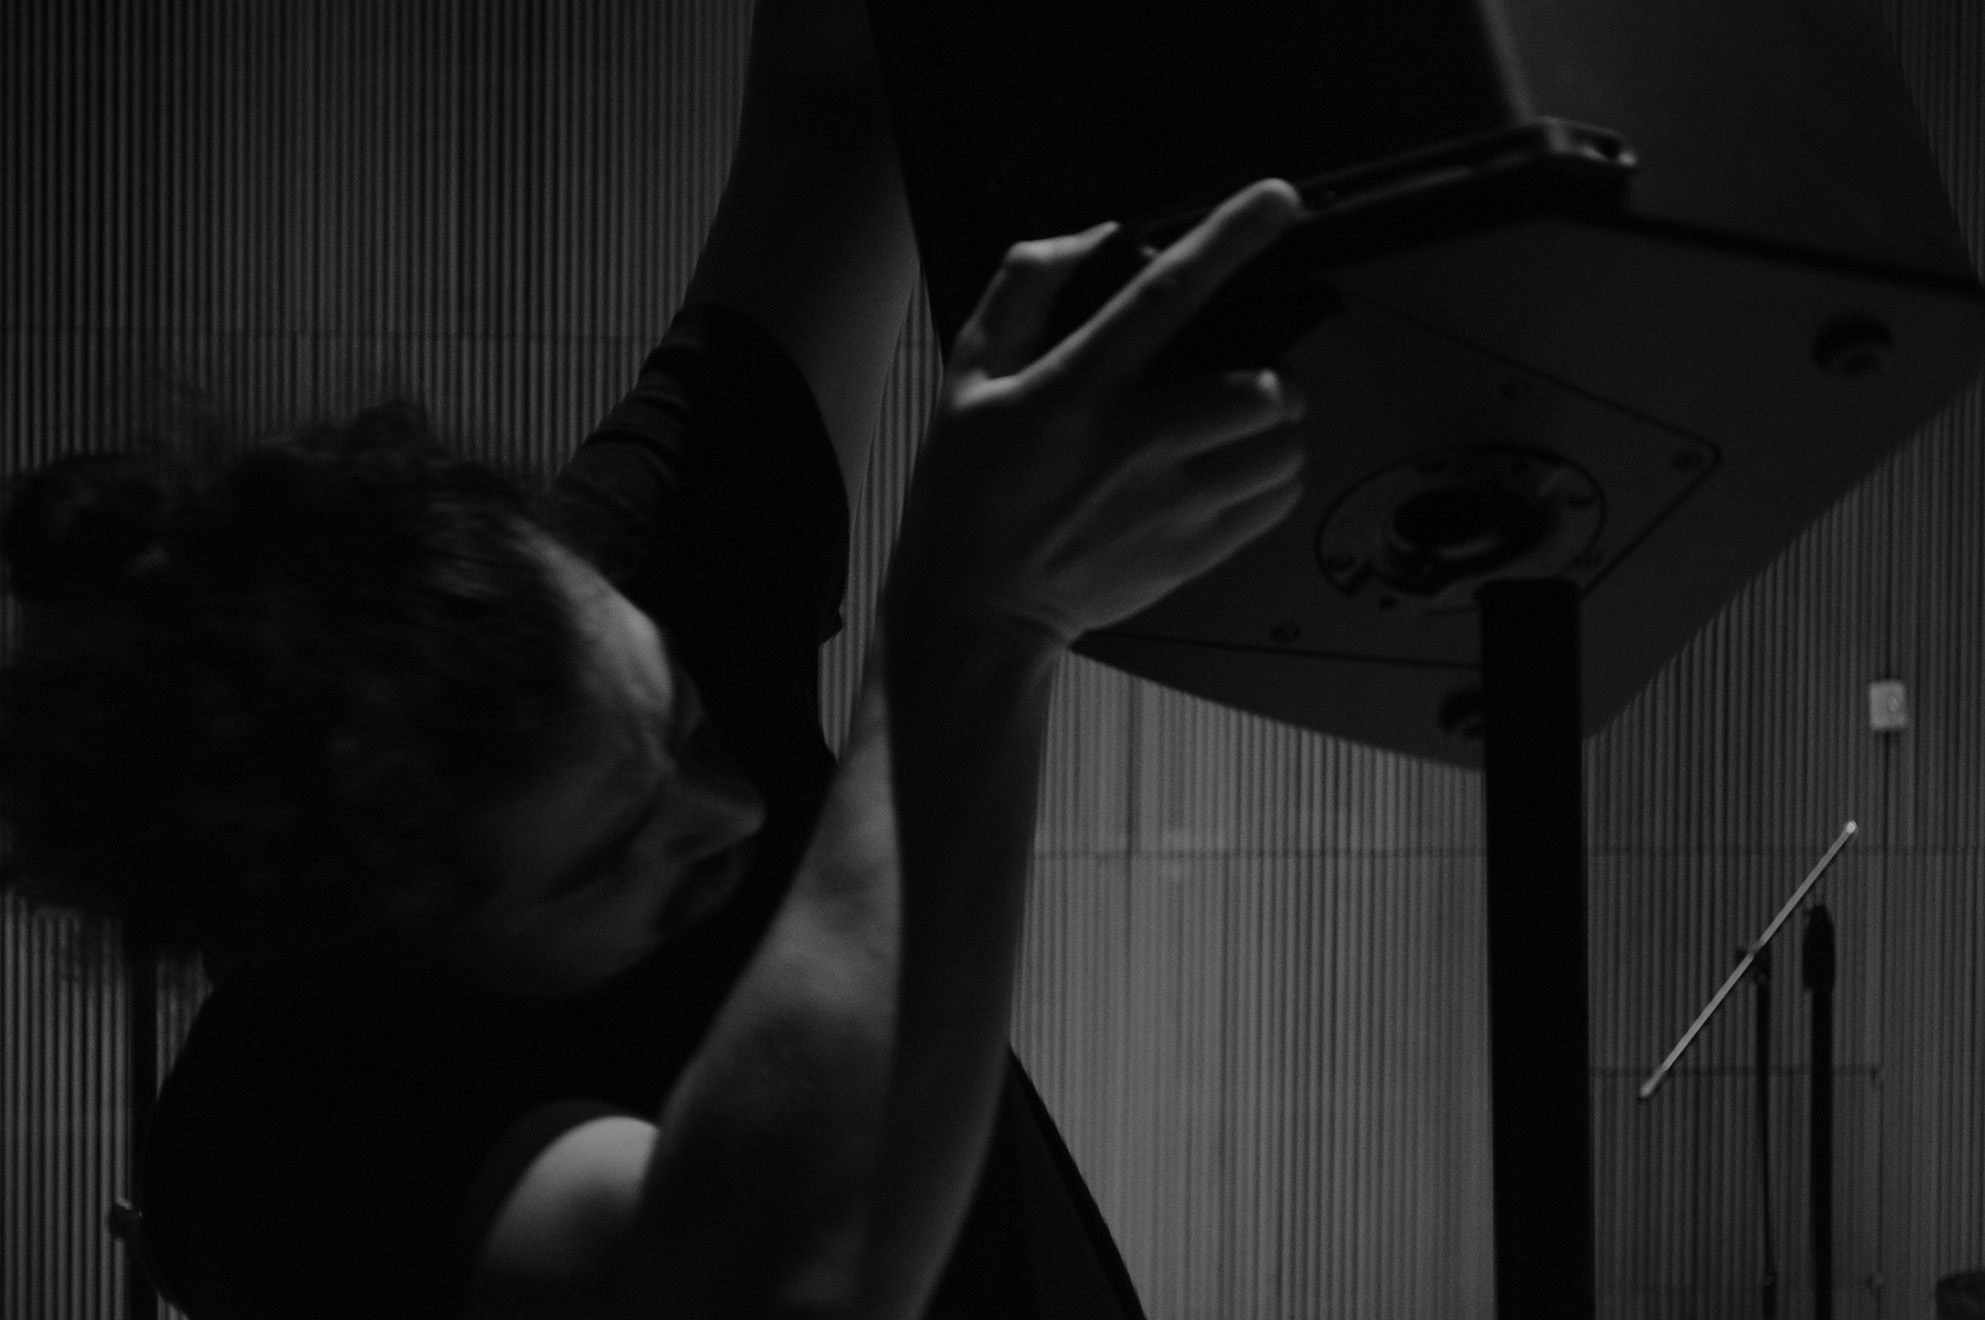
\includegraphics[height=8cm]{fdch.jpg}
\subsection{full name}
federico nicolás cámara halac
\subsection{date of birth}
may 8th, 1988
\subsection{country of birth}
argentina
\subsection{mailing address}
24 waverly place r.268. new york, ny 10003. usa
\subsection{phone}
(1) 347-302-0982
\subsection{e-mail}
camarafede@gmail.com / fch226@nyu.edu
\subsection{website}
\href{http://fdch.github.io/tv}{fdch.github.io/tv}
\newpage
\section{education}
\subsection{graduate education}
phd candiate in music composition. nyu gsas music department (2013-)
\subsection{undergraduate education}
licentiate in music composition at the faculty of arts, national university of córdoba, argentina (2006-12)
\section{teaching}
\subsection{professor}
\begin{itemize}
\item harmony and counterpoint i, nyu fas. fall (2015)
\end{itemize}
\subsection{teaching}
\begin{itemize}
\item computer music theory and techniques. nyu fas. fall (2016)
\item harmony and counterpoint ii, nyu fas. spring (2015)
\item harmony and counterpoint i, nyu fas. fall (2014)
\item music composition i, unc. national university of cordoba (2009-10)
\item aural perception i, unc. national university of cordoba (2007-08)
\end{itemize}
 
\section{awards}
\subsection{fellowships}
\begin{itemize}
\item gri fellowship (graduate research initiative) for research based in paris (2017)
\item maccracken fellowship (nyu, graduate school of arts and science, music department) (2013-2018)
\item programa cuarto centenario, for an exchange at l'université de montréal to study c++ (2012)
\end{itemize}
\subsection{prizes}
\begin{itemize}
\item his work \href{http://fedecamarahalac.com/lagos.php }{lagos}, for orchestra, was selected for premiere by the unc orchestra, 2011 (cba, arg).
\item works selected by the destellos foundation: \href{http://fedecamarahalac.com/ciudad.php" }{ciudad invertida} (2015) and \href{http://fedecamarahalac.com/venas.php" }{venas} (2014)
\end{itemize}
\section{work}
\subsection{2017}
\begin{itemize}
\item a.le.a, for talea ensemble, live video and electronics (10’)
\end{itemize}
\subsection{2016}
\begin{itemize}
\item i[n, for scapegoat ensemble with live amplification (15’)
\item sk, for tak ensemble (15-20’)
\item canon, for proyecto[red]ensamble with five performers and potentiometers (7’)
\item inopera, for loadbang ensemble (43’)
\end{itemize}
\subsection{2015}
\begin{itemize}
\item ciudad invertida / inverted city, for trombone duo, live video and electronics (12’)
\item huesos / bones, for four percussionists (15-20’)
\item venas / veins, for bass clarinet live video and electronics (10’)
\item flesh / carne, for bass clarinet, cello, percussion, double bass and piano (8’)
\item study duchamp, electroacoustic (5’)
\end{itemize}
\subsection{2014}
\begin{itemize}
\item venas / veins, for bass clarinet and electronics (8’)
\item talita, for string quartet and video (12’)
\end{itemize}
\subsection{2013}
\begin{itemize}
\item la linea imposible del horizonte / the impossible line of the horizon, for ensemble (8’)
\item aponia for choir and piano (7’)
\item cloud relations for string quartet and fixed electronics (13’)
\end{itemize}
\subsection{2012}
\begin{itemize}
\item el alargamiento de las sombras / the elonging of the shadows, for chamber septet (8’)
\item memories for esther for solo piano (7’)
\item un tiempo en utopia / a time in utopia for choir and large ensemble (18’)
\end{itemize}
\subsection{2011}
\begin{itemize}
\item piano and ensemble: water symmetries no2 (10’)
\item water symmetries no1 for reed quintet (12’)
\item viola for solo viola (6’)
\item lagos / lakes, for full symphony orchestra (12’)
\item piano, fagot y guitarra for piano, bassoon and guitar (10’)
\end{itemize}
\subsection{2010}
\begin{itemize}
\item 11 variaciones / 11 variations, for piano (10’)
\item instantáneas / instantaneous, for soprano (w/text) and ensemble (9’)
\item móvil-in-móvil / mobile-im-mobile, for two percussionists, piano and electro-acoustic (8‘)
\item niebla dorada / golden fog, for soprano and ensemble, based on texts from árbol de diana, by alejandra pizarnik (10’ 30’’)
\end{itemize}
\subsection{2009}
\begin{itemize}
\item three to nine from slap!, for wind ensemble (6’)
\item three for slap!, for reed quintet (6’)
\item 2 movimientos / 2 movements, for string quartet (5’ 27’’)
\item keys for flute and prepared piano (2’ 50’’)
\item tensiones (tensions) for solo percussion (3’)
\item música para arpa solo (music for solo harp) (4’)
\end{itemize}
\subsection{2008}
\begin{itemize}
\item sixty for piano (2’)
\item she dwelt among the untrodden ways for voice and piano, based on william wordsworth’s homonymous poem (3’)
\item meditación para mezzo-soprano (meditation for mezzo-soprano), based on a sentence by oscar wilde (2’)
\end{itemize}
\subsection{2007}
\begin{itemize}
\item suite for violin and piano (10’)
\end{itemize}

\subsection{artistic code}
<h6>externals written in c for pure data</h6>
\begin{itemize}
\item <code>lorenz.c</code> outputs the lorenz system of equations
\item <code>siginfo.c</code> analyzes a 3 dimensional system of coordinates
\item <code>minimax.c</code> outputs minimum and maximum values of a list
\item <code>crand.c</code> runs the c native prng
\item <code>mtwister.c</code> runs takuji nishimura's 1997 code for a prng using mersenne primes
\end{itemize}

\section{collaborations}
\subsection{dance}
\begin{itemize}
\item assisting josé halac’s musicalization gómez-comini’s ballet “alicia en el país de las maravillas”. teatro san martín, cba (2010)
\end{itemize}
\subsection{film}
\begin{itemize}
\item original soundtrack composition and recording of lauro racosky’s “al cielo o al infierno”. gran rex movie theaters. this film received a special award for best film trailer in the mar del plata film festival. the trailer was syncronized with the original music composition (2011)
\end{itemize}

\subsection{theatre}
\begin{itemize}
\item “itinerante: un viaje a través de los sentidos”. electroacoustics and sound art for muñoz and rosencovich’s undergraduate final thesis. cba (2012)
\item “nueva sub ciudad”. electroacoustic composition for luisina couto’s undergraduate final thesis (2011)
\item electroacoustic composition for lozada and echeverría’s version of pavlovsky’s “poroto”. pabellón azul, unc, cba (2013)
\item original score for luisina couto’s play inserto beat. cineclub municipal, cba (2010)
\end{itemize}
\subsection{opera}
\begin{itemize}
\item “los chicos de abril” by composer luis perez. fixed electronics in collaboration with pablo behm and franco pellini. rio cuarto municipal theatre, cba (2013)
\end{itemize}
\subsection{participation in ensembles and orchestras}
\begin{itemize}
\item nov. 2012. faculty of arts’ aniversary. piano in five (john cage), and trumpet in ensamble para hormigas amigas (pablo behm). cepia auditorium; 
\item p[r]e concert: piano in los tan conocidos flechazos (manuel pastrana), the elonging of the shadows (federico cámara halac) and módulos (josé llorens). cepia auditorium;
\item sept. 2012. john cage festival. piano in one and five (john cage), with proyecto[red]ensamble. cepia auditorium;
\item aug. 2012. b2cim. piano in memories for esther cepia auditorium; p[r]e concert. trumpet and midi controller in ensamble para hormigas amigas (pablo behm).
\item jun. 2012. final composition thesis and alchemists’ concert: piano in piano, bassoon and guitar. cepia auditorium, fcefyn auditorium;
\item oct. 2011. congress for human sciences. electric guitar in electric counterpoint (steve reich). monserrat school;
\item sept. 2011. musical analysis micro-symposiums. piano in movin’ (ariel contreras). open rehearsal. faculty of arts;
\item aug. 2011. 2nd forum for the arts. homage to oscar bazán. piano in los mitos (oscar bazán) cepia auditorium;
\item jul. 2011: winter concert. elec. guitar in electric counterpoint, piano in los mitos, trío (1958) (césar m. franchisena), and piano, fagot y guitarra. cepia auditorium;
\item nov. 2010: summer concert. conductor in instantáneas, piano in ciudad sin sueño (nocturno del brooklyn bridge) (pablo behm), injection (cecilia quiroga), afluentes (pablo rojas) and such (miguel stamburgo) cepia auditorium;
\item jul. 2010, the machine of time - cycle. trumpet in con voce (mauricio kagel). spain/cordoba cultural center.
pianist improviser: leim ensemble. belonging to the faculty of arts and the cepia, this project is dedicated to the collective, real-time creation of sound discourse with instruments and electronics:
\item aug. 2012. experimentalia 2012. midi controller. ccec auditorium;
\item nov. 2011. summer concert. cepia auditorium;
\item oct. 2011. teatro acústico (acoustic theatre) with composer/conductor oscar edelstein (bs.as). faculty of arts;
\item sept. 2011. musical analysis micro-symposiums. faculty of arts;
\item sept. 2011. contengo-arte - cycle. institute in cordoba;
\item aug. 2011. winter concert. cepia auditorium;
\item jun. 2011. experimentalia 2011 - cycle spain/cordoba cultural center;
\item may 2011. new music and sound art encounter: tsonami 2011. buenos aires, recoleta cultural center; dec. 2010. leim in concert. spain/cordoba cultural center;
\item nov. 2010. summer concert, cepia auditorium;
\item sept. 2010. 1st international biennial of music composition and education, cepia auditorium.
\item guest pianist: lamoi. rock band. performances in march, may and november 2012. pianist in the band’s first record, recorded in july 2012. the disc premiered on april 2013.
\item guest pianist: rio ceballos symphony orchestra. performances in march, may and november 2010. guitarist: cast member of the theatre play inserto beat.
\end{itemize}

\tableofcontents

\end{document}
